\documentclass{article}
% NeurIPS template; "preprint" removes line numbers and the anonymous-submission banner.
\usepackage[preprint]{neurips_2025}
\makeatletter\renewcommand{\@noticestring}{NLP 097215 Final Project (Track 1), Technion, 2026.
Code: \url{https://github.com/htmldanielpoly/nlp_final_project}; weights: \url{https://huggingface.co/htmldaniel/reading-agent-multabench}.}\makeatother

\usepackage[utf8]{inputenc}
\usepackage[T1]{fontenc}
\usepackage{hyperref}
\usepackage{url}
\usepackage{booktabs}
\usepackage{amsfonts,amsmath,amssymb}
\usepackage{nicefrac}
\usepackage{microtype}
\usepackage{xcolor}
\usepackage{graphicx}
\usepackage{tikz}
\usetikzlibrary{arrows.meta,positioning,calc}

\newcommand{\nRuns}{100}
\newcommand{\nFolds}{5}
\newcommand{\minFolds}{5}
\newcommand{\maxFolds}{5}
\newcommand{\meanBlendCls}{0.900}
\newcommand{\meanReadAllCls}{0.893}
\newcommand{\meanCBFrozenCls}{0.887}
\newcommand{\meanTableOnlyCls}{0.751}
\newcommand{\blendVsLocalCBClsDelta}{+0.012}
\newcommand{\blendVsLocalCBClsWins}{10}
\newcommand{\blendVsLocalCBClsP}{0.002}
\newcommand{\blendVsLbCBFrozenClsDelta}{+0.011}
\newcommand{\blendVsLbCBFrozenClsWins}{10}
\newcommand{\blendVsLbCBFrozenClsP}{0.002}
\newcommand{\blendVsLbCBTarClsDelta}{$-$0.008}
\newcommand{\blendVsLbCBTarClsWins}{3}
\newcommand{\blendVsLbCBTarClsP}{0.049}
\newcommand{\blendVsReadAllClsDelta}{+0.007}
\newcommand{\blendVsReadAllClsWins}{10}
\newcommand{\blendVsReadAllClsP}{0.002}
\newcommand{\readAllVsLbCBFrozenClsDelta}{+0.004}
\newcommand{\readAllVsLbCBFrozenClsWins}{5}
\newcommand{\readAllVsLbCBTarClsDelta}{$-$0.015}
\newcommand{\readAllVsLbCBTarClsWins}{0}
\newcommand{\readAllVsLocalCBClsDelta}{+0.005}
\newcommand{\readAllVsLocalCBClsWins}{6}
\newcommand{\gainContentTenClsDelta}{+0.026}
\newcommand{\gainContentTenClsWins}{9}
\newcommand{\gainContentTenClsP}{0.031}
\newcommand{\gainContentQuarterClsDelta}{+0.024}
\newcommand{\gainContentQuarterClsWins}{9}
\newcommand{\gainContentQuarterClsP}{0.031}
\newcommand{\gainMetaTenClsDelta}{+0.010}
\newcommand{\gainMetaTenClsWins}{8}
\newcommand{\gainMetaTenClsP}{0.031}
\newcommand{\gainMetaQuarterClsDelta}{+0.018}
\newcommand{\gainMetaQuarterClsWins}{8}
\newcommand{\gainMetaQuarterClsP}{0.031}
\newcommand{\meanBlendReg}{0.702}
\newcommand{\meanReadAllReg}{0.640}
\newcommand{\meanCBFrozenReg}{0.684}
\newcommand{\meanTableOnlyReg}{0.422}
\newcommand{\blendVsLocalCBRegDelta}{+0.017}
\newcommand{\blendVsLocalCBRegWins}{8}
\newcommand{\blendVsLocalCBRegP}{0.008}
\newcommand{\blendVsLbCBFrozenRegDelta}{+0.008}
\newcommand{\blendVsLbCBFrozenRegWins}{9}
\newcommand{\blendVsLbCBFrozenRegP}{0.064}
\newcommand{\blendVsLbCBTarRegDelta}{$-$0.014}
\newcommand{\blendVsLbCBTarRegWins}{2}
\newcommand{\blendVsLbCBTarRegP}{0.027}
\newcommand{\blendVsReadAllRegDelta}{+0.062}
\newcommand{\blendVsReadAllRegWins}{10}
\newcommand{\blendVsReadAllRegP}{0.002}
\newcommand{\readAllVsLbCBFrozenRegDelta}{$-$0.053}
\newcommand{\readAllVsLbCBFrozenRegWins}{2}
\newcommand{\readAllVsLbCBTarRegDelta}{$-$0.075}
\newcommand{\readAllVsLbCBTarRegWins}{0}
\newcommand{\readAllVsLocalCBRegDelta}{$-$0.044}
\newcommand{\readAllVsLocalCBRegWins}{3}
\newcommand{\gainContentTenRegDelta}{+0.051}
\newcommand{\gainContentTenRegWins}{10}
\newcommand{\gainContentTenRegP}{0.016}
\newcommand{\gainContentQuarterRegDelta}{+0.053}
\newcommand{\gainContentQuarterRegWins}{10}
\newcommand{\gainContentQuarterRegP}{0.016}
\newcommand{\gainMetaTenRegDelta}{+0.037}
\newcommand{\gainMetaTenRegWins}{10}
\newcommand{\gainMetaTenRegP}{0.016}
\newcommand{\gainMetaQuarterRegDelta}{+0.039}
\newcommand{\gainMetaQuarterRegWins}{9}
\newcommand{\gainMetaQuarterRegP}{0.018}
\newcommand{\recN}{19}
\newcommand{\recContentTen}{63\%}
\newcommand{\recRandomContentTen}{39\%}
\newcommand{\recContentQuarter}{81\%}
\newcommand{\recRandomContentQuarter}{58\%}
\newcommand{\recMetaTen}{45\%}
\newcommand{\recRandomMetaTen}{24\%}
\newcommand{\recMetaQuarter}{71\%}
\newcommand{\recRandomMetaQuarter}{52\%}
\newcommand{\recMaxP}{$<$0.001}
\newcommand{\rhoTextEffectCls}{0.50}
\newcommand{\rhoTextEffectClsP}{0.138}
\newcommand{\rhoTextEffectReg}{0.75}
\newcommand{\rhoTextEffectRegP}{0.013}
\newcommand{\sFakeJobPostingReadAll}{0.901}
\newcommand{\sFakeJobPostingCBFrozen}{0.893}
\newcommand{\sFakeJobPostingBlend}{0.911}
\newcommand{\sFakeJobPostingTableOnly}{0.672}
\newcommand{\sFakeJobPostingCBTab}{0.679}
\newcommand{\sFakeJobPostingLbCBTar}{0.912}
\newcommand{\sFakeJobPostingLbTabMFrozen}{0.933}
\newcommand{\sFakeJobPostingLbBestTar}{0.929}
\newcommand{\sFakeJobPostingLbBestFrozen}{0.945}
\newcommand{\sJigsawToxicityReadAll}{0.868}
\newcommand{\sJigsawToxicityCBFrozen}{0.819}
\newcommand{\sJigsawToxicityBlend}{0.870}
\newcommand{\sJigsawToxicityTableOnly}{0.551}
\newcommand{\sJigsawToxicityCBTab}{0.566}
\newcommand{\sJigsawToxicityLbCBTar}{0.927}
\newcommand{\sJigsawToxicityLbTabMFrozen}{0.799}
\newcommand{\sJigsawToxicityLbBestTar}{0.937}
\newcommand{\sJigsawToxicityLbBestFrozen}{0.834}
\newcommand{\sKickstarterReadAll}{0.734}
\newcommand{\sKickstarterCBFrozen}{0.729}
\newcommand{\sKickstarterBlend}{0.744}
\newcommand{\sKickstarterTableOnly}{0.646}
\newcommand{\sKickstarterCBTab}{0.654}
\newcommand{\sKickstarterLbCBTar}{0.744}
\newcommand{\sKickstarterLbTabMFrozen}{0.740}
\newcommand{\sKickstarterLbBestTar}{0.752}
\newcommand{\sKickstarterLbBestFrozen}{0.744}
\newcommand{\sDsSalaryReadAll}{0.826}
\newcommand{\sDsSalaryCBFrozen}{0.822}
\newcommand{\sDsSalaryBlend}{0.831}
\newcommand{\sDsSalaryTableOnly}{0.553}
\newcommand{\sDsSalaryCBTab}{0.554}
\newcommand{\sDsSalaryLbCBTar}{0.828}
\newcommand{\sDsSalaryLbTabMFrozen}{0.836}
\newcommand{\sDsSalaryLbBestTar}{0.839}
\newcommand{\sDsSalaryLbBestFrozen}{0.837}
\newcommand{\sMichelinReadAll}{0.904}
\newcommand{\sMichelinCBFrozen}{0.906}
\newcommand{\sMichelinBlend}{0.912}
\newcommand{\sMichelinTableOnly}{0.867}
\newcommand{\sMichelinCBTab}{0.874}
\newcommand{\sMichelinLbCBTar}{0.917}
\newcommand{\sMichelinLbTabMFrozen}{0.912}
\newcommand{\sMichelinLbBestTar}{0.925}
\newcommand{\sMichelinLbBestFrozen}{0.915}
\newcommand{\sProductSentimentReadAll}{0.904}
\newcommand{\sProductSentimentCBFrozen}{0.893}
\newcommand{\sProductSentimentBlend}{0.906}
\newcommand{\sProductSentimentTableOnly}{0.819}
\newcommand{\sProductSentimentCBTab}{0.826}
\newcommand{\sProductSentimentLbCBTar}{0.914}
\newcommand{\sProductSentimentLbTabMFrozen}{0.899}
\newcommand{\sProductSentimentLbBestTar}{0.925}
\newcommand{\sProductSentimentLbBestFrozen}{0.918}
\newcommand{\sSpotifyGenresReadAll}{0.957}
\newcommand{\sSpotifyGenresCBFrozen}{0.960}
\newcommand{\sSpotifyGenresBlend}{0.967}
\newcommand{\sSpotifyGenresTableOnly}{0.912}
\newcommand{\sSpotifyGenresCBTab}{0.922}
\newcommand{\sSpotifyGenresLbCBTar}{0.964}
\newcommand{\sSpotifyGenresLbTabMFrozen}{0.959}
\newcommand{\sSpotifyGenresLbBestTar}{0.964}
\newcommand{\sSpotifyGenresLbBestFrozen}{0.960}
\newcommand{\sUsAccidentsReadAll}{0.957}
\newcommand{\sUsAccidentsCBFrozen}{0.971}
\newcommand{\sUsAccidentsBlend}{0.972}
\newcommand{\sUsAccidentsTableOnly}{0.861}
\newcommand{\sUsAccidentsCBTab}{0.903}
\newcommand{\sUsAccidentsLbCBTar}{0.977}
\newcommand{\sUsAccidentsLbTabMFrozen}{0.971}
\newcommand{\sUsAccidentsLbBestTar}{0.982}
\newcommand{\sUsAccidentsLbBestFrozen}{0.979}
\newcommand{\sWineReviewReadAll}{0.977}
\newcommand{\sWineReviewCBFrozen}{0.975}
\newcommand{\sWineReviewBlend}{0.979}
\newcommand{\sWineReviewTableOnly}{0.856}
\newcommand{\sWineReviewCBTab}{0.857}
\newcommand{\sWineReviewLbCBTar}{0.981}
\newcommand{\sWineReviewLbTabMFrozen}{0.978}
\newcommand{\sWineReviewLbBestTar}{0.982}
\newcommand{\sWineReviewLbBestFrozen}{0.978}
\newcommand{\sWomenClothingReadAll}{0.898}
\newcommand{\sWomenClothingCBFrozen}{0.903}
\newcommand{\sWomenClothingBlend}{0.905}
\newcommand{\sWomenClothingTableOnly}{0.773}
\newcommand{\sWomenClothingCBTab}{0.780}
\newcommand{\sWomenClothingLbCBTar}{0.909}
\newcommand{\sWomenClothingLbTabMFrozen}{0.907}
\newcommand{\sWomenClothingLbBestTar}{0.913}
\newcommand{\sWomenClothingLbBestFrozen}{0.909}
\newcommand{\sBabiesPricesReadAll}{0.824}
\newcommand{\sBabiesPricesCBFrozen}{0.866}
\newcommand{\sBabiesPricesBlend}{0.875}
\newcommand{\sBabiesPricesTableOnly}{0.399}
\newcommand{\sBabiesPricesCBTab}{0.385}
\newcommand{\sBabiesPricesLbCBTar}{0.893}
\newcommand{\sBabiesPricesLbTabMFrozen}{0.900}
\newcommand{\sBabiesPricesLbBestTar}{0.927}
\newcommand{\sBabiesPricesLbBestFrozen}{0.914}
\newcommand{\sBookPriceReadAll}{0.364}
\newcommand{\sBookPriceCBFrozen}{0.517}
\newcommand{\sBookPriceBlend}{0.519}
\newcommand{\sBookPriceTableOnly}{0.191}
\newcommand{\sBookPriceCBTab}{0.212}
\newcommand{\sBookPriceLbCBTar}{0.565}
\newcommand{\sBookPriceLbTabMFrozen}{0.560}
\newcommand{\sBookPriceLbBestTar}{0.565}
\newcommand{\sBookPriceLbBestFrozen}{0.570}
\newcommand{\sBookReadabilityReadAll}{0.820}
\newcommand{\sBookReadabilityCBFrozen}{0.815}
\newcommand{\sBookReadabilityBlend}{0.831}
\newcommand{\sBookReadabilityTableOnly}{0.790}
\newcommand{\sBookReadabilityCBTab}{0.782}
\newcommand{\sBookReadabilityLbCBTar}{0.829}
\newcommand{\sBookReadabilityLbTabMFrozen}{0.816}
\newcommand{\sBookReadabilityLbBestTar}{0.844}
\newcommand{\sBookReadabilityLbBestFrozen}{0.832}
\newcommand{\sMercariReadAll}{0.374}
\newcommand{\sMercariCBFrozen}{0.433}
\newcommand{\sMercariBlend}{0.444}
\newcommand{\sMercariTableOnly}{0.097}
\newcommand{\sMercariCBTab}{0.099}
\newcommand{\sMercariLbCBTar}{0.450}
\newcommand{\sMercariLbTabMFrozen}{0.454}
\newcommand{\sMercariLbBestTar}{0.471}
\newcommand{\sMercariLbBestFrozen}{0.473}
\newcommand{\sMontgomerySalReadAll}{0.964}
\newcommand{\sMontgomerySalCBFrozen}{0.976}
\newcommand{\sMontgomerySalBlend}{0.975}
\newcommand{\sMontgomerySalTableOnly}{0.961}
\newcommand{\sMontgomerySalCBTab}{0.974}
\newcommand{\sMontgomerySalLbCBTar}{0.975}
\newcommand{\sMontgomerySalLbTabMFrozen}{0.975}
\newcommand{\sMontgomerySalLbBestTar}{0.984}
\newcommand{\sMontgomerySalLbBestFrozen}{0.979}
\newcommand{\sRottenTomatoesReadAll}{0.497}
\newcommand{\sRottenTomatoesCBFrozen}{0.493}
\newcommand{\sRottenTomatoesBlend}{0.524}
\newcommand{\sRottenTomatoesTableOnly}{0.183}
\newcommand{\sRottenTomatoesCBTab}{0.190}
\newcommand{\sRottenTomatoesLbCBTar}{0.521}
\newcommand{\sRottenTomatoesLbTabMFrozen}{0.531}
\newcommand{\sRottenTomatoesLbBestTar}{0.573}
\newcommand{\sRottenTomatoesLbBestFrozen}{0.556}
\newcommand{\sScimagoImpactReadAll}{0.854}
\newcommand{\sScimagoImpactCBFrozen}{0.870}
\newcommand{\sScimagoImpactBlend}{0.873}
\newcommand{\sScimagoImpactTableOnly}{0.730}
\newcommand{\sScimagoImpactCBTab}{0.737}
\newcommand{\sScimagoImpactLbCBTar}{0.875}
\newcommand{\sScimagoImpactLbTabMFrozen}{0.879}
\newcommand{\sScimagoImpactLbBestTar}{0.888}
\newcommand{\sScimagoImpactLbBestFrozen}{0.880}
\newcommand{\sVancouverSalReadAll}{0.732}
\newcommand{\sVancouverSalCBFrozen}{0.754}
\newcommand{\sVancouverSalBlend}{0.769}
\newcommand{\sVancouverSalTableOnly}{0.306}
\newcommand{\sVancouverSalCBTab}{0.314}
\newcommand{\sVancouverSalLbCBTar}{0.788}
\newcommand{\sVancouverSalLbTabMFrozen}{0.766}
\newcommand{\sVancouverSalLbBestTar}{0.798}
\newcommand{\sVancouverSalLbBestFrozen}{0.792}
\newcommand{\sVideoGamesReadAll}{0.366}
\newcommand{\sVideoGamesCBFrozen}{0.295}
\newcommand{\sVideoGamesBlend}{0.381}
\newcommand{\sVideoGamesTableOnly}{0.036}
\newcommand{\sVideoGamesCBTab}{0.038}
\newcommand{\sVideoGamesLbCBTar}{0.419}
\newcommand{\sVideoGamesLbTabMFrozen}{0.485}
\newcommand{\sVideoGamesLbBestTar}{0.506}
\newcommand{\sVideoGamesLbBestFrozen}{0.485}
\newcommand{\sZomatoReadAll}{0.608}
\newcommand{\sZomatoCBFrozen}{0.825}
\newcommand{\sZomatoBlend}{0.825}
\newcommand{\sZomatoTableOnly}{0.523}
\newcommand{\sZomatoCBTab}{0.575}
\newcommand{\sZomatoLbCBTar}{0.840}
\newcommand{\sZomatoLbTabMFrozen}{0.844}
\newcommand{\sZomatoLbBestTar}{0.862}
\newcommand{\sZomatoLbBestFrozen}{0.865}

% written by `python -m reading_agent.controls_report --tag controls_v2 --fieldmeta_tag fieldmeta_v1 --out ../paper/generated`
\IfFileExists{generated/controls.tex}{\newcommand{\ctlFolds}{5}
\newcommand{\ctlDatasets}{20}
\newcommand{\ctlTotalContentTenClsDelta}{+0.053}
\newcommand{\ctlTotalContentTenClsWins}{10}
\newcommand{\ctlTotalContentTenClsN}{10}
\newcommand{\ctlTotalContentTenClsP}{0.016}
\newcommand{\ctlTotalMetaTenClsDelta}{+0.020}
\newcommand{\ctlTotalMetaTenClsWins}{8}
\newcommand{\ctlTotalMetaTenClsN}{10}
\newcommand{\ctlTotalMetaTenClsP}{0.059}
\newcommand{\ctlChoiceContentTenClsDelta}{+0.027}
\newcommand{\ctlChoiceContentTenClsWins}{9}
\newcommand{\ctlChoiceContentTenClsN}{10}
\newcommand{\ctlChoiceContentTenClsP}{0.031}
\newcommand{\ctlChoiceMetaTenClsDelta}{+0.014}
\newcommand{\ctlChoiceMetaTenClsWins}{9}
\newcommand{\ctlChoiceMetaTenClsN}{10}
\newcommand{\ctlChoiceMetaTenClsP}{0.031}
\newcommand{\ctlAllocContentTenClsDelta}{+0.027}
\newcommand{\ctlAllocContentTenClsWins}{10}
\newcommand{\ctlAllocContentTenClsN}{10}
\newcommand{\ctlAllocContentTenClsP}{0.016}
\newcommand{\ctlAllocMetaTenClsDelta}{+0.005}
\newcommand{\ctlAllocMetaTenClsWins}{8}
\newcommand{\ctlAllocMetaTenClsN}{10}
\newcommand{\ctlAllocMetaTenClsP}{0.420}
\newcommand{\ctlNaturalContentTenClsDelta}{+0.044}
\newcommand{\ctlNaturalContentTenClsWins}{10}
\newcommand{\ctlNaturalContentTenClsN}{10}
\newcommand{\ctlNaturalContentTenClsP}{0.016}
\newcommand{\ctlNaturalMetaTenClsDelta}{+0.009}
\newcommand{\ctlNaturalMetaTenClsWins}{6}
\newcommand{\ctlNaturalMetaTenClsN}{10}
\newcommand{\ctlNaturalMetaTenClsP}{1.000}
\newcommand{\ctlTotalContentTenRegDelta}{+0.122}
\newcommand{\ctlTotalContentTenRegWins}{10}
\newcommand{\ctlTotalContentTenRegN}{10}
\newcommand{\ctlTotalContentTenRegP}{0.016}
\newcommand{\ctlTotalMetaTenRegDelta}{+0.086}
\newcommand{\ctlTotalMetaTenRegWins}{10}
\newcommand{\ctlTotalMetaTenRegN}{10}
\newcommand{\ctlTotalMetaTenRegP}{0.016}
\newcommand{\ctlChoiceContentTenRegDelta}{+0.051}
\newcommand{\ctlChoiceContentTenRegWins}{10}
\newcommand{\ctlChoiceContentTenRegN}{10}
\newcommand{\ctlChoiceContentTenRegP}{0.016}
\newcommand{\ctlChoiceMetaTenRegDelta}{+0.038}
\newcommand{\ctlChoiceMetaTenRegWins}{10}
\newcommand{\ctlChoiceMetaTenRegN}{10}
\newcommand{\ctlChoiceMetaTenRegP}{0.016}
\newcommand{\ctlAllocContentTenRegDelta}{+0.071}
\newcommand{\ctlAllocContentTenRegWins}{10}
\newcommand{\ctlAllocContentTenRegN}{10}
\newcommand{\ctlAllocContentTenRegP}{0.016}
\newcommand{\ctlAllocMetaTenRegDelta}{+0.048}
\newcommand{\ctlAllocMetaTenRegWins}{10}
\newcommand{\ctlAllocMetaTenRegN}{10}
\newcommand{\ctlAllocMetaTenRegP}{0.016}
\newcommand{\ctlNaturalContentTenRegDelta}{+0.123}
\newcommand{\ctlNaturalContentTenRegWins}{10}
\newcommand{\ctlNaturalContentTenRegN}{10}
\newcommand{\ctlNaturalContentTenRegP}{0.016}
\newcommand{\ctlNaturalMetaTenRegDelta}{+0.088}
\newcommand{\ctlNaturalMetaTenRegWins}{10}
\newcommand{\ctlNaturalMetaTenRegN}{10}
\newcommand{\ctlNaturalMetaTenRegP}{0.016}
\newcommand{\fmTableClsWithout}{0.753}
\newcommand{\fmTableClsWith}{0.778}
\newcommand{\fmTableClsDelta}{+0.025}
\newcommand{\fmTableClsWins}{9}
\newcommand{\fmTableClsN}{10}
\newcommand{\fmTableClsP}{0.014}
\newcommand{\fmReadallClsWithout}{0.889}
\newcommand{\fmReadallClsWith}{0.887}
\newcommand{\fmReadallClsDelta}{$-$0.002}
\newcommand{\fmReadallClsWins}{3}
\newcommand{\fmReadallClsN}{10}
\newcommand{\fmReadallClsP}{0.232}
\newcommand{\fmAdvContentTenClsWithout}{+0.028}
\newcommand{\fmAdvContentTenClsWith}{+0.017}
\newcommand{\fmAdvContentTenClsDelta}{$-$0.011}
\newcommand{\fmAdvContentTenClsWins}{1}
\newcommand{\fmAdvContentTenClsN}{10}
\newcommand{\fmAdvContentTenClsP}{0.012}
\newcommand{\fmAdvContentQuarterClsWithout}{+0.023}
\newcommand{\fmAdvContentQuarterClsWith}{+0.017}
\newcommand{\fmAdvContentQuarterClsDelta}{$-$0.006}
\newcommand{\fmAdvContentQuarterClsWins}{1}
\newcommand{\fmAdvContentQuarterClsN}{10}
\newcommand{\fmAdvContentQuarterClsP}{0.008}
\newcommand{\fmAdvMetaTenClsWithout}{+0.016}
\newcommand{\fmAdvMetaTenClsWith}{+0.009}
\newcommand{\fmAdvMetaTenClsDelta}{$-$0.007}
\newcommand{\fmAdvMetaTenClsWins}{1}
\newcommand{\fmAdvMetaTenClsN}{10}
\newcommand{\fmAdvMetaTenClsP}{0.020}
\newcommand{\fmAdvMetaQuarterClsWithout}{+0.018}
\newcommand{\fmAdvMetaQuarterClsWith}{+0.015}
\newcommand{\fmAdvMetaQuarterClsDelta}{$-$0.002}
\newcommand{\fmAdvMetaQuarterClsWins}{3}
\newcommand{\fmAdvMetaQuarterClsN}{10}
\newcommand{\fmAdvMetaQuarterClsP}{0.164}
\newcommand{\fmTableRegWithout}{0.430}
\newcommand{\fmTableRegWith}{0.467}
\newcommand{\fmTableRegDelta}{+0.037}
\newcommand{\fmTableRegWins}{8}
\newcommand{\fmTableRegN}{10}
\newcommand{\fmTableRegP}{0.020}
\newcommand{\fmReadallRegWithout}{0.671}
\newcommand{\fmReadallRegWith}{0.645}
\newcommand{\fmReadallRegDelta}{$-$0.026}
\newcommand{\fmReadallRegWins}{2}
\newcommand{\fmReadallRegN}{10}
\newcommand{\fmReadallRegP}{0.105}
\newcommand{\fmAdvContentTenRegWithout}{+0.051}
\newcommand{\fmAdvContentTenRegWith}{+0.064}
\newcommand{\fmAdvContentTenRegDelta}{+0.013}
\newcommand{\fmAdvContentTenRegWins}{8}
\newcommand{\fmAdvContentTenRegN}{10}
\newcommand{\fmAdvContentTenRegP}{0.232}
\newcommand{\fmAdvContentQuarterRegWithout}{+0.054}
\newcommand{\fmAdvContentQuarterRegWith}{+0.065}
\newcommand{\fmAdvContentQuarterRegDelta}{+0.010}
\newcommand{\fmAdvContentQuarterRegWins}{4}
\newcommand{\fmAdvContentQuarterRegN}{10}
\newcommand{\fmAdvContentQuarterRegP}{1.000}
\newcommand{\fmAdvMetaTenRegWithout}{+0.034}
\newcommand{\fmAdvMetaTenRegWith}{+0.028}
\newcommand{\fmAdvMetaTenRegDelta}{$-$0.006}
\newcommand{\fmAdvMetaTenRegWins}{5}
\newcommand{\fmAdvMetaTenRegN}{10}
\newcommand{\fmAdvMetaTenRegP}{0.625}
\newcommand{\fmAdvMetaQuarterRegWithout}{+0.040}
\newcommand{\fmAdvMetaQuarterRegWith}{+0.023}
\newcommand{\fmAdvMetaQuarterRegDelta}{$-$0.017}
\newcommand{\fmAdvMetaQuarterRegWins}{2}
\newcommand{\fmAdvMetaQuarterRegN}{10}
\newcommand{\fmAdvMetaQuarterRegP}{0.014}
}{}
\newcommand{\htab}{h_{\mathrm{tab}}}
\setlength{\textfloatsep}{10pt plus 2pt minus 4pt}
\setlength{\floatsep}{8pt plus 2pt minus 2pt}

\title{Reading What Matters: Table-Conditioned Selective\\Text Reading for Text-Tabular Prediction}

\author{Daniel Polyanovsky\\Technion -- Israel Institute of Technology}

\begin{document}
\maketitle

\begin{abstract}
Text-tabular models encode \emph{every} text field of a row, although the structured columns often already determine the prediction and only some rows need some of their text.
We propose a \emph{reading agent}: a table encoder initialises a recurrent \emph{anytime} reader that consumes frozen-E5 sentence items one at a time and can predict after any number of reads, and an \emph{expected-gain head}, adapted from dynamic feature selection, reads greedily while the predicted loss reduction exceeds a cost $\lambda$.
On all 20 text datasets of MulTaBench (five splits each), learned reading significantly beats a random reader with the same per-row budget at every budget we test, e.g.\ by \gainContentTenClsDelta{} AUROC and \gainContentTenRegDelta{} $R^2$ at a nominal 10\% of the retained text items.
For full-budget accuracy, a validation-tuned blend of the reader with a CatBoost Joint-Frozen model significantly improves on CatBoost Joint Frozen (\blendVsLocalCBClsDelta{} AUROC, \blendVsLocalCBRegDelta{} $R^2$) but does not reach the Joint TAR baselines.
We report this gap, a negative result for imitation learning, and where adaptive reading does and does not help.
\end{abstract}

%======================================================================
\section{Introduction}

In text-tabular learning, a row combines numerical and categorical columns with free-text fields such as reviews or job descriptions~\cite{arazi2026multabench}.
Standard practice embeds each field with a pretrained encoder such as E5~\cite{wang2022e5} and trains a tabular learner on the result (\emph{Joint Frozen}), or fine-tunes the encoder on the target (\emph{Joint TAR})~\cite{arazi2025tabstar,arazi2026multabench}.
Both treat all text as equally necessary for every row.
Human analysts read differently: if a wine's price and region already pin down its grade, the review is worth reading only when the table leaves the answer ambiguous, and then one sentence may suffice.
We turn this into an algorithm: the structured part of a row initialises a recurrent reader, which acquires text one \emph{item} (a field-tagged sentence chunk) at a time, choosing the item with the highest predicted loss reduction, until that gain no longer pays for the reading cost.

\paragraph{Contributions.}
(i)~A table-conditioned anytime reader for text-tabular rows, trained with random reading orders so it is valid after any subset of reads.
(ii)~A reading policy, label-free at inference, that regresses observed one-step loss reductions, in the spirit of DIME~\cite{gadgil2024dime}, in two access modes: \emph{content} keys (routing over already-embedded text) and \emph{metadata} keys (field and position only, so unread content is not inspected for selection).
(iii)~An evaluation on all 20 MulTaBench text datasets with paired local baselines and dataset-level statistics.
(iv)~Analyses of where adaptive reading helps, and a negative result for imitating a label oracle.

%======================================================================
\section{Related Work}

\textbf{Text-tabular learning.}
MulTaBench~\cite{arazi2026multabench} curates datasets on which text and structure are jointly needed and target-aware representations help.
It evaluates CatBoost~\cite{prokhorenkova2018catboost}, LightGBM~\cite{ke2017lightgbm}, TabM~\cite{gorishniy2024tabm} and TabPFN~\cite{hollmann2025tabpfn,grinsztajn2025tabpfn25} with frozen or LoRA-tuned~\cite{hu2022lora} E5 embeddings.
TabSTAR~\cite{arazi2025tabstar} unfreezes the text encoder inside a tabular foundation model, and CARTE~\cite{kim2024carte} embeds column names and strings for transfer.
Shi et al.~\cite{shi2021multimodal} show that ensembling neural text models with tabular learners is strong; our blend follows that practice and is not claimed as novel.
\textbf{Dynamic feature selection.}
Active feature acquisition chooses which features to observe per instance~\cite{shim2018afa}.
Covert et al.~\cite{covert2023dfs} learn greedy information-maximising policies without RL, and DIME~\cite{gadgil2024dime} regresses the reduction in prediction loss and stops at a threshold.
Our gain head applies DIME's estimator to field-tagged text chunks, with a table-derived prior state.
\textbf{Adaptive reading.}
LSTM-Jump~\cite{yu2017skim} and Skim-RNN~\cite{seo2018skimrnn} learn to skip or skim tokens of one document, and adaptive computation time~\cite{graves2016act} learns how many recurrent steps to spend; we select among a tabular row's fields and chunks, conditioned on its columns.

%======================================================================
\section{Method}

\begin{figure}[t]
\centering
\resizebox{\linewidth}{!}{%
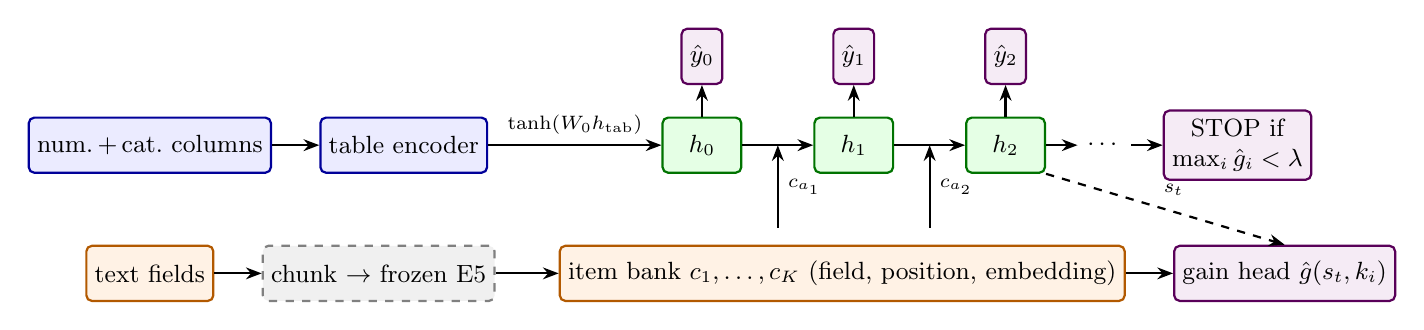
\begin{tikzpicture}[node distance=4mm and 6mm,
  bx/.style={draw, rounded corners=2pt, thick, align=center, minimum height=7mm, inner sep=3pt, font=\small},
  tb/.style={bx, draw=blue!60!black, fill=blue!8},
  tx/.style={bx, draw=orange!70!black, fill=orange!10},
  rn/.style={bx, draw=green!45!black, fill=green!10, minimum width=10mm},
  hd/.style={bx, draw=violet!70!black, fill=violet!8},
  fz/.style={bx, draw=gray, fill=gray!12, dashed},
  ar/.style={-{Stealth[length=2mm]}, thick}]
  \node[tb] (row) {num.\,+\,cat.\ columns};
  \node[tb, right=of row] (enc) {table encoder};
  \node[rn, right=22mm of enc] (h0) {$h_0$};
  \node[rn, right=9mm of h0] (h1) {$h_1$};
  \node[rn, right=9mm of h1] (h2) {$h_2$};
  \node[font=\small, right=4mm of h2] (dots) {$\cdots$};
  \node[hd, right=4mm of dots] (stop) {STOP if\\$\max_i \hat g_i<\lambda$};
  \foreach \t in {0,1,2} { \node[hd, above=4mm of h\t] (y\t) {$\hat y_\t$}; \draw[ar] (h\t) -- (y\t); }
  \draw[ar] (row) -- (enc); \draw[ar] (enc) -- node[above, font=\scriptsize]{$\tanh(W_0\htab)$} (h0);
  \draw[ar] (h0) -- (h1); \draw[ar] (h1) -- (h2); \draw[ar] (h2) -- (dots); \draw[ar] (dots) -- (stop);
  \node[tx, below=9mm of row] (txt) {text fields};
  \node[fz, right=of txt] (e5) {chunk $\to$ frozen E5};
  \node[tx, right=8mm of e5, minimum width=40mm] (bank) {item bank $c_1,\dots,c_K$ (field, position, embedding)};
  \node[hd, right=6mm of bank] (gain) {gain head $\hat g(s_t,k_i)$};
  \draw[ar] (txt) -- (e5); \draw[ar] (e5) -- (bank); \draw[ar] (bank) -- (gain);
  \draw[ar] ($(h0)!0.5!(h1)+(0,-1.05)$) -- node[right, font=\scriptsize]{$c_{a_1}$} ($(h0)!0.5!(h1)$);
  \draw[ar] ($(h1)!0.5!(h2)+(0,-1.05)$) -- node[right, font=\scriptsize]{$c_{a_2}$} ($(h1)!0.5!(h2)$);
  \draw[ar, dashed] (h2.south east) -- node[above right, pos=0.45, font=\scriptsize]{$s_t$} (gain.north);
\end{tikzpicture}}
\caption{The reading agent: the table initialises a 2-layer GRU; at each step the gain head scores unread items, the reader consumes the best one, and $\hat y_t$ is available after every step.}
\label{fig:arch}
\end{figure}

\textbf{Text items.}
Each text field is split into sentences, merged or cut into chunks of at most 48 words (a field's chunks beyond the eighth merge into one tail item, which E5 truncates at 512 tokens).
Items are allocated round-robin across fields up to $K=\max(8,\#\text{fields})$ per row, so every field has at least one item; the kept items contain every word of the row on 13 of the 20 datasets, before encoder truncation (coverage: Appendix~\ref{app:cov}).
Each item is verbalised as \texttt{passage: <column>: <chunk>} and embedded once with frozen E5-small-v2~\cite{wang2022e5} ($e_i\in\mathbb{R}^{384}$, cached).
Inside the model, an item is
$c_i=\mathrm{LN}(W_{\text{item}}e_i + W_{\text{name}}\,\mathrm{E5}(\text{field name}) + p_{\text{pos}(i)})\in\mathbb{R}^{128}$.

\textbf{Table encoder and anytime reader.}
Numerical columns are quantile-normalised.
Each column becomes a token $x_jw_j+m_ju_j+n_j$ (numerical; $m_j$ marks missingness) or $\mathrm{Emb}(v_j)+n_j$ (categorical), where $n_j$ is a projected E5 embedding of the column name.
The flattened tokens pass through an MLP to $\htab\in\mathbb{R}^{128}$, which initialises both layers of a GRU~\cite{cho2014gru} (Fig.~\ref{fig:arch}).
After reading items $a_1,\dots,a_t$, the state is $s_t=[h^{(2)}_t;\ \tfrac1t\sum_{\tau\le t}c_{a_\tau};\ \htab]$ (the mean term is zero at $t=0$), and an MLP predictor outputs $f(s_t)$.
We train the encoder, reader and predictor together, sampling a fresh random reading order per batch:
\begin{equation}
\mathcal{L}_{\text{read}}=\tfrac12\cdot\tfrac{1}{n+1}\textstyle\sum_{t=0}^{n}\ell\big(f(s_t),y\big)+\tfrac12\,\ell\big(f(s_n),y\big),
\end{equation}
where $n\le K$ is the row's number of items, $\ell$ is cross-entropy for classification and MSE on the standardised target for regression.
Random orders make $f$ a valid predictor after \emph{any} subset of reads, which the policy relies on.

\textbf{Expected-gain policy.}
With the reader frozen, a head $\hat g(s_t,k_i)=\mathrm{MLP}([s_t;k_i])$ predicts the loss reduction from reading item $i$ next.
The \emph{content} key is $k_i=c_i$.
The \emph{metadata} key uses only the field and position embeddings, so the content of unread text is never inspected.
On a held-out inner-validation split we roll in $\varepsilon$-greedily ($\varepsilon=0.3$) with the current head, in the DAgger style~\cite{ross2011dagger}, so training states match the states the policy visits.
At every visited state we compute the observed gain of every unread item and regress it:
\begin{equation}
\Delta_i(s_t)=\ell\big(f(s_t),y\big)-\ell\big(f(s_t\oplus c_i),y\big),\qquad
\mathcal{L}_{\text{gain}}=\textstyle\sum_{t}\sum_{i\ \text{unread}}\big(\hat g(s_t,k_i)-\Delta_i(s_t)\big)^2 .
\end{equation}
The label only builds targets: at test time $\hat g$ estimates $\mathbb{E}[\Delta_i\mid s_t,k_i]$ without $y$, a predicted improvement of \emph{our} predictor's loss rather than an exact information estimate.
\textbf{Inference:} read $\arg\max_i\hat g$ while $\max_i \hat g\ge\lambda$.
For a target fraction of items read (10/25/50/75\%), we bisect $\lambda$ on the validation split.
This needs only $\hat g$, not labels.

\textbf{Why not imitation? (negative result).}
Our first policy, a pointer network imitating a greedy oracle that reads the item most reducing the loss for the \emph{true} label, was no better than random in pilots: plausibly because the oracle's choices depend on $y$ (it reached 0.966 AUROC on Women Clothing with 1.5 reads per row), which the policy cannot see; regressing the \emph{expected} gain avoids this.

\textbf{Full-budget accuracy mode.}
For the benchmark objective we combine the read-all reader with a CatBoost Joint-Frozen model built from the same E5 cache (structured columns + PCA-30 of each field's whole-text E5 embedding).
The convex weight $w\in\{0,0.05,\dots,1\}$ is tuned on inner validation.
The reader learns target-trained projections of the text embeddings, so we treat \textbf{Joint TAR as the relevant bar} and also report Joint Frozen.

%======================================================================
\section{Experiments}

\paragraph{Setup.}
We use all 20 MulTaBench text datasets (10 classification, binary or macro one-vs-rest AUROC; 10 regression, $R^2$) under the paper protocol: random holdout splits (seed $42+$fold, test capped at 2{,}000 and train at 10{,}000 rows) ported from the official \texttt{paper\_version} code; five splits per dataset.
An inner 80/20 split of the outer training set provides validation for early stopping (100 epochs, patience 15), the gain head, $\lambda$ and the blend weight; pilots informed the architecture, but the recipe was fixed before the five-split evaluation.
All datasets share one configuration ($d=128$, dropout 0.2, AdamW lr $10^{-3}$, batch 256; gain head 15 epochs, lr $3\cdot10^{-3}$).
Local CatBoost baselines share our exact rows; external references are the official leaderboard scores for the same split seeds (row identity unverified, so they are approximate references without significance tests).
Following Dem\v{s}ar~\cite{demsar2006statistical}, we average folds within each dataset and run two-sided Wilcoxon signed-rank tests over datasets, separately for AUROC and $R^2$.

\begin{table}[t]
\caption{Full-budget accuracy, dataset means (folds averaged per dataset).
W/T/L: datasets where the Blend wins, ties or loses against that row; $^{*}$: two-sided Wilcoxon $p<0.05$ (local rows only).
$^{\dagger n}$: reference for only $n$ datasets; [ ]: the Blend's mean on those $n$.}
\label{tab:main}
\centering
\footnotesize
\begin{tabular}{@{}lcccc@{}}
\toprule
 & \multicolumn{2}{c}{Classification (10, AUROC)} & \multicolumn{2}{c}{Regression (10, $R^2$)} \\
\cmidrule(lr){2-3}\cmidrule(lr){4-5}
Method & mean & Blend W/T/L & mean & Blend W/T/L \\
\midrule
\multicolumn{5}{@{}l}{\emph{Ours}} \\
Reader, table only (0 reads) & 0.751 & 10/0/0$^{*}$ & 0.422 & 10/0/0$^{*}$ \\
Reader, read all & 0.893 & 10/0/0$^{*}$ & 0.640 & 10/0/0$^{*}$ \\
\textbf{Blend}: CatBoost Frozen + reader & 0.900 &  & 0.702 &  \\
\midrule
\multicolumn{5}{@{}l}{\emph{Local baselines (identical rows)}} \\
CatBoost, tabular only & 0.762 & 10/0/0$^{*}$ & 0.430 & 10/0/0$^{*}$ \\
CatBoost, Joint Frozen & 0.887 & 10/0/0$^{*}$ & 0.684 & 8/1/1$^{*}$ \\
\midrule
\multicolumn{5}{@{}l}{\emph{MulTaBench reference, Joint Frozen (E5)}} \\
CatBoost, Joint Frozen & 0.889 & 10/0/0 & 0.693 & 9/0/1 \\
LightGBM, Joint Frozen & 0.872 & 10/0/0 & 0.675 & 10/0/0 \\
TabM, Joint Frozen & 0.893 & 7/0/3 & 0.721 & 3/0/7 \\
TabPFN-2.5, Joint Frozen & 0.885$^{\dagger8}$\,[0.881] & 2/0/6 & 0.727 & 0/0/10 \\
\midrule
\multicolumn{5}{@{}l}{\emph{MulTaBench reference, Joint TAR (LoRA-tuned E5)}} \\
CatBoost, Joint TAR & 0.907 & 3/0/7 & 0.716 & 2/0/8 \\
LightGBM, Joint TAR & 0.894 & 7/0/3 & 0.702 & 6/0/4 \\
TabM, Joint TAR & 0.911 & 2/0/8 & 0.728 & 1/0/9 \\
TabPFN-2.5, Joint TAR & 0.900$^{\dagger8}$\,[0.881] & 0/0/8 & 0.732 & 0/0/10 \\
\bottomrule
\end{tabular}

\end{table}

\paragraph{Full-budget accuracy (Table~\ref{tab:main}).}
The blend improves on CatBoost Joint Frozen on both families, against our local run on identical rows (\blendVsLocalCBClsDelta{} AUROC with \blendVsLocalCBClsWins/10 wins, $p=\blendVsLocalCBClsP$; \blendVsLocalCBRegDelta{} $R^2$ with \blendVsLocalCBRegWins/10 wins, $p=\blendVsLocalCBRegP$); against the leaderboard's CatBoost Frozen reference it wins on \blendVsLbCBFrozenClsWins/10 and \blendVsLbCBFrozenRegWins/10 datasets.
Without fold 0, which pilots also used, the gains are +0.013 and +0.017 (both $p<0.01$).
It does \emph{not} reach Joint TAR (\blendVsLbCBTarClsDelta{} AUROC and \blendVsLbCBTarRegDelta{} $R^2$ against CatBoost TAR; TabM and TabPFN-2.5 are stronger still), so the objective of beating Joint TAR is \textbf{not met}.
The reader alone is competitive with CatBoost Frozen on classification (\readAllVsLocalCBClsDelta{} AUROC) but weaker on regression (\readAllVsLocalCBRegDelta{} $R^2$); their errors differ, which is why the blend helps (per-dataset results: Appendix~\ref{app:per}).
The reader wins clearly when text carries most of the signal (Video Games $R^2$ \sVideoGamesReadAll{} vs.\ \sVideoGamesCBFrozen{} for CatBoost Frozen; Jigsaw AUROC \sJigsawToxicityReadAll{} vs.\ \sJigsawToxicityCBFrozen) and loses most on Zomato (\sZomatoReadAll{} vs.\ \sZomatoCBFrozen), whose rows average 1{,}900 words, of which the $K$ items keep only 6\%.

\begin{figure}[t]
\centering
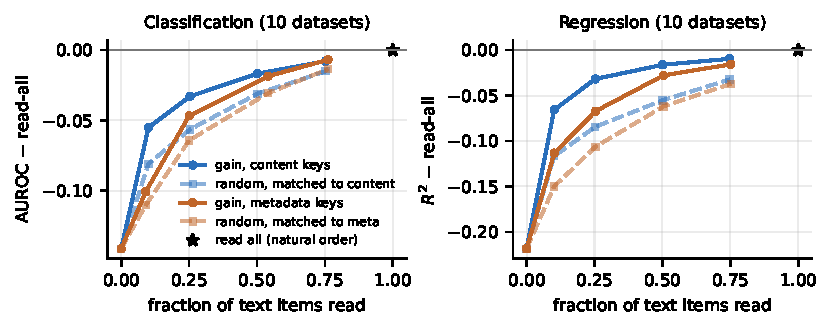
\includegraphics[width=0.56\linewidth]{generated/fig_budget.pdf}
\caption{Score minus read-all score (dataset means) vs.\ fraction of items read. Solid: gain policy; dashed: random reader with the same per-row reads (3 orders); $\star$: read-all, natural order.}
\label{fig:budget}
\end{figure}

\begin{table}[t]
\caption{Gain policy minus matched-random reader per nominal budget (dataset level). ``read'': mean achieved test fraction; $p_{\text{Holm}}$: Wilcoxon $p$, Holm-adjusted~\cite{holm1979} over the 8 key$\times$budget cells per family.}
\label{tab:budget}
\centering
\footnotesize
\setlength{\tabcolsep}{4pt}
\begin{tabular}{@{}llcccccccc@{}}
\toprule
 & & \multicolumn{4}{c}{Classification ($\Delta$AUROC)} & \multicolumn{4}{c}{Regression ($\Delta R^2$)} \\
\cmidrule(lr){3-6}\cmidrule(lr){7-10}
Keys & Budget & read & $\Delta$ & W/T/L & $p_{\text{Holm}}$ & read & $\Delta$ & W/T/L & $p_{\text{Holm}}$ \\
\midrule
content & 10\% & 10\% & +0.026 & 9/1/0 & 0.031 & 10\% & +0.051 & 10/0/0 & 0.016 \\
content & 25\% & 25\% & +0.024 & 9/1/0 & 0.031 & 25\% & +0.053 & 10/0/0 & 0.016 \\
content & 50\% & 50\% & +0.014 & 9/1/0 & 0.031 & 50\% & +0.039 & 10/0/0 & 0.016 \\
content & 75\% & 75\% & +0.007 & 9/1/0 & 0.031 & 75\% & +0.023 & 9/0/1 & 0.018 \\
\midrule
metadata & 10\% & 9\% & +0.010 & 8/1/1 & 0.031 & 10\% & +0.037 & 10/0/0 & 0.016 \\
metadata & 25\% & 25\% & +0.018 & 8/1/1 & 0.031 & 25\% & +0.039 & 9/0/1 & 0.018 \\
metadata & 50\% & 54\% & +0.012 & 8/1/1 & 0.031 & 50\% & +0.034 & 9/0/1 & 0.018 \\
metadata & 75\% & 76\% & +0.007 & 9/1/0 & 0.031 & 75\% & +0.021 & 9/0/1 & 0.016 \\
\bottomrule
\end{tabular}

\end{table}

\paragraph{Selective reading (Fig.~\ref{fig:budget}, Table~\ref{tab:budget}).}
At 10\% of the items the content policy beats the matched random reader by \gainContentTenClsDelta{} AUROC (\gainContentTenClsWins/10 datasets) and \gainContentTenRegDelta{} $R^2$ (\gainContentTenRegWins/10); all 16 key$\times$budget comparisons are significant after Holm correction.
The random reader gets the policy's per-row read counts, isolating \emph{which} items are read (and in what order) from \emph{how many}.
Against random items with the same \emph{total} reads spread over rows by item count (Appendix~\ref{app:ctl}), the 10\% gap widens to \ctlTotalContentTenClsDelta{} AUROC and \ctlTotalContentTenRegDelta{} $R^2$ (\ctlTotalContentTenClsWins/10 and \ctlTotalContentTenRegWins/10): at small budgets choosing \emph{which rows} to read matters as much as which items, and stored field order is barely better than random.
Metadata keys, which never see unread content, also win at every budget with smaller margins (\gainMetaTenClsDelta{} AUROC, \gainMetaTenRegDelta{} $R^2$ at 10\%).
Discrete gain scores make some nominal budgets unattainable (Table~\ref{tab:budget}); only metadata keys could avoid embedding unread items.

\paragraph{Where reading helps.}
At 10\% of the items the content policy recovers a median \recContentTen{} of what reading everything adds over the table alone, against \recRandomContentTen{} for the matched random reader (metadata keys: \recMetaTen{} vs.\ \recRandomMetaTen; \recN{} datasets where text adds $\ge$0.02, Wilcoxon $p\,\recMaxP$).
The advantage grows with how much the text helps (Spearman $\rho=\rhoTextEffectReg$, $p=\rhoTextEffectRegP$ on regression; $\rho=\rhoTextEffectCls$, $p=\rhoTextEffectClsP$ on classification), rather than simply with text length: it is largest on Rotten Tomatoes (+0.14 $R^2$), Vancouver Salaries (+0.11) and DS Salary (+0.085 AUROC), and near zero where the table decides (Montgomery Salaries) or rows hold 1--2 items (Product Sentiment, Jigsaw).
Giving the table encoder each field's presence and log length (Appendix~\ref{app:ctl}) raises table-only scores (\fmTableClsDelta{} AUROC, \fmTableRegDelta{} $R^2$) and shrinks the 10\% content advantage on classification (\fmAdvContentTenClsWithout{}$\to$\fmAdvContentTenClsWith) but not regression (\fmAdvContentTenRegWithout{}$\to$\fmAdvContentTenRegWith): reading is partly, not only, ``read the long fields''.

%======================================================================
\section{Conclusion}

On 20 MulTaBench text datasets, table-conditioned selective reading with a DIME-style gain policy significantly beats budget-matched random reading at every budget, even with metadata-only keys; blended with CatBoost Joint Frozen, the reader improves on it but does not reach Joint TAR.
\textbf{Limitations:} a simple MLP table encoder holds back the full-budget reader (weak on regression); the gain head is one-step greedy; the inner validation split is reused for stopping, gain fitting and calibration; the $K$-item cap drops long text (Zomato).
\textbf{Future work:} a stronger table backbone (e.g.\ TabM), lexical previews before E5 encoding, and LoRA-tuned item encoders.

\bibliographystyle{plain}
\bibliography{references}

\appendix
\makeatletter\setlength{\@fptop}{0pt}\setlength{\@fpsep}{12pt plus 1fil}\makeatother % top-align appendix float pages
\section{Per-dataset results}\label{app:per}
\begin{table}[h]
\caption{Fold-mean scores per dataset. CB: our CatBoost (tab: tabular only).
R: reader (table only / gain policy, content keys, @25\% / read all).
Blend $\pm$ fold std.
LB: MulTaBench leaderboard for matching split seeds (row identity unverified); best TAR is the maximum over the four learners.
Bold: best of our columns.}
\centering
\scriptsize
\setlength{\tabcolsep}{3pt}
\resizebox{\linewidth}{!}{\begin{tabular}{@{}lcccccccccc@{}}
\toprule
Dataset & folds & CB tab & CB Frozen & R: table & R: gain@25\% & R: all & Blend & LB CB Frozen & LB CB TAR & LB best TAR \\
\midrule
\multicolumn{11}{@{}l}{\emph{Classification (AUROC)}} \\
Fake Job Posting & 5 & 0.679 & 0.893 & 0.672 & 0.851 & 0.901 & \textbf{0.911}\tiny{$\pm$0.019} & 0.906 & 0.912 & 0.929 \\
Jigsaw Toxicity & 5 & 0.566 & 0.819 & 0.551 & 0.760 & 0.868 & \textbf{0.870}\tiny{$\pm$0.021} & 0.818 & 0.927 & 0.937 \\
Kickstarter & 5 & 0.654 & 0.729 & 0.646 & 0.711 & 0.734 & \textbf{0.744}\tiny{$\pm$0.012} & 0.729 & 0.744 & 0.752 \\
DS Salary & 5 & 0.554 & 0.822 & 0.553 & 0.798 & 0.826 & \textbf{0.831}\tiny{$\pm$0.006} & 0.820 & 0.828 & 0.839 \\
Michelin & 5 & 0.874 & 0.906 & 0.867 & 0.894 & 0.904 & \textbf{0.912}\tiny{$\pm$0.004} & 0.905 & 0.917 & 0.925 \\
Product Sentiment & 5 & 0.826 & 0.893 & 0.819 & 0.855 & 0.904 & \textbf{0.906}\tiny{$\pm$0.005} & 0.900 & 0.914 & 0.925 \\
Spotify Genres & 5 & 0.922 & 0.960 & 0.912 & 0.946 & 0.957 & \textbf{0.967}\tiny{$\pm$0.002} & 0.960 & 0.964 & 0.964 \\
US Accidents & 5 & 0.903 & 0.971 & 0.861 & 0.952 & 0.957 & \textbf{0.972}\tiny{$\pm$0.005} & 0.971 & 0.977 & 0.982 \\
Wine Review & 5 & 0.857 & 0.975 & 0.856 & 0.955 & 0.977 & \textbf{0.979}\tiny{$\pm$0.001} & 0.975 & 0.981 & 0.982 \\
Women Clothing & 5 & 0.780 & 0.903 & 0.773 & 0.874 & 0.898 & \textbf{0.905}\tiny{$\pm$0.003} & 0.903 & 0.909 & 0.913 \\
\midrule
\multicolumn{11}{@{}l}{\emph{Regression ($R^2$)}} \\
Babies Prices & 5 & 0.385 & 0.866 & 0.399 & 0.786 & 0.824 & \textbf{0.875}\tiny{$\pm$0.038} & 0.872 & 0.893 & 0.927 \\
Book Price & 5 & 0.212 & 0.517 & 0.191 & 0.305 & 0.364 & \textbf{0.519}\tiny{$\pm$0.032} & 0.543 & 0.565 & 0.565 \\
Book Readability & 5 & 0.782 & 0.815 & 0.790 & 0.811 & 0.820 & \textbf{0.831}\tiny{$\pm$0.018} & 0.819 & 0.829 & 0.844 \\
Mercari & 5 & 0.099 & 0.433 & 0.097 & 0.332 & 0.374 & \textbf{0.444}\tiny{$\pm$0.026} & 0.436 & 0.450 & 0.471 \\
Montgomery Sal. & 5 & 0.974 & \textbf{0.976} & 0.961 & 0.963 & 0.964 & 0.975\tiny{$\pm$0.007} & 0.972 & 0.975 & 0.984 \\
Rotten Tomatoes & 5 & 0.190 & 0.493 & 0.183 & 0.462 & 0.497 & \textbf{0.524}\tiny{$\pm$0.030} & 0.508 & 0.521 & 0.573 \\
SCImago Impact & 5 & 0.737 & 0.870 & 0.730 & 0.841 & 0.854 & \textbf{0.873}\tiny{$\pm$0.007} & 0.868 & 0.875 & 0.888 \\
Vancouver Sal. & 5 & 0.314 & 0.754 & 0.306 & 0.659 & 0.732 & \textbf{0.769}\tiny{$\pm$0.028} & 0.764 & 0.788 & 0.798 \\
Video Games & 5 & 0.038 & 0.295 & 0.036 & 0.333 & 0.366 & \textbf{0.381}\tiny{$\pm$0.130} & 0.325 & 0.419 & 0.506 \\
Zomato & 5 & 0.575 & \textbf{0.825} & 0.523 & 0.591 & 0.608 & \textbf{0.825}\tiny{$\pm$0.006} & 0.825 & 0.840 & 0.862 \\
\bottomrule
\end{tabular}
}
\end{table}

\clearpage
\section{Text coverage of the item representation}\label{app:cov}
\begin{table}[!ht]
\caption{Fold-0 test rows. Items/row: items kept after the cap $K$; rows over $K$: rows with more candidate chunks than $K$; words kept: share of the row's words inside kept items (an upper bound on what E5 sees, since a field's chunks beyond the eighth are merged into one and E5 truncates at 512 tokens).}
\centering
\scriptsize
\begin{tabular}{@{}lcccccc@{}}
\toprule
Dataset & text fields & $K$ & words/row & items/row & rows over $K$ & words kept \\
\midrule
\multicolumn{7}{@{}l}{\emph{Classification}} \\
Fake Job Posting & 3 & 8 & 176 & 5.4 & 15\% & 89\% \\
Jigsaw Toxicity & 1 & 8 & 52 & 1.8 & 0\% & 100\% \\
Kickstarter & 3 & 8 & 26 & 3.0 & 0\% & 100\% \\
DS Salary & 5 & 8 & 29 & 4.8 & 0\% & 100\% \\
Michelin & 6 & 8 & 110 & 7.4 & 17\% & 94\% \\
Product Sentiment & 1 & 8 & 18 & 1.0 & 0\% & 100\% \\
Spotify Genres & 3 & 8 & 9 & 3.0 & 0\% & 100\% \\
US Accidents & 6 & 8 & 19 & 6.0 & 0\% & 100\% \\
Wine Review & 2 & 8 & 41 & 2.2 & 0\% & 100\% \\
Women Clothing & 2 & 8 & 62 & 2.7 & 0\% & 100\% \\
\midrule
\multicolumn{7}{@{}l}{\emph{Regression}} \\
Babies Prices & 4 & 8 & 12 & 2.7 & 0\% & 100\% \\
Book Price & 5 & 8 & 176 & 7.4 & 43\% & 77\% \\
Book Readability & 6 & 8 & 185 & 7.8 & 49\% & 90\% \\
Mercari & 6 & 8 & 37 & 5.8 & 1\% & 99\% \\
Montgomery Sal. & 3 & 8 & 9 & 3.0 & 0\% & 100\% \\
Rotten Tomatoes & 13 & 13 & 71 & 12.8 & 1\% & 100\% \\
SCImago Impact & 10 & 10 & 28 & 10.0 & 0\% & 100\% \\
Vancouver Sal. & 2 & 8 & 5 & 2.0 & 0\% & 100\% \\
Video Games & 2 & 8 & 6 & 2.0 & 0\% & 100\% \\
Zomato & 7 & 8 & 1909 & 7.8 & 79\% & 6\% \\
\bottomrule
\end{tabular}

\end{table}

\IfFileExists{generated/tab_controls.tex}{%
\section{Reading controls}\label{app:ctl}
\begin{table}[!ht]
\caption{Dataset-level mean difference (wins/datasets) at nominal budgets 10\% and 50\%, all five folds (folds averaged per dataset).
\emph{Same total reads}: random items, with the policy's total number of reads spread over rows in proportion to their item counts.
\emph{Same per-row reads}: random items with the policy's per-row counts (as in Table~\ref{tab:budget}).
\emph{Row allocation}: the second random reader minus the first.
\emph{Natural order}: fields and chunks in their stored order, same counts as the first reader.
$^{*}$: Holm-adjusted Wilcoxon $p<0.05$ over the eight key$\times$budget cells.}
\centering
\scriptsize
\setlength{\tabcolsep}{3pt}
\begin{tabular}{@{}llcccc@{}}
\toprule
 & & \multicolumn{2}{c}{Classification ($\Delta$AUROC)} & \multicolumn{2}{c}{Regression ($\Delta R^2$)} \\
\cmidrule(lr){3-4}\cmidrule(lr){5-6}
Comparison & Keys & 10\% & 50\% & 10\% & 50\% \\
\midrule
gain $-$ random (same total reads) & content & +0.053 (10/10)$^{*}$ & +0.019 (10/10)$^{*}$ & +0.122 (10/10)$^{*}$ & +0.068 (10/10)$^{*}$ \\
 & metadata & +0.020 (8/10) & +0.015 (8/10) & +0.086 (10/10)$^{*}$ & +0.060 (10/10)$^{*}$ \\
\midrule
gain $-$ random (same per-row reads) & content & +0.027 (9/10)$^{*}$ & +0.014 (9/10)$^{*}$ & +0.051 (10/10)$^{*}$ & +0.042 (10/10)$^{*}$ \\
 & metadata & +0.014 (9/10)$^{*}$ & +0.013 (8/10)$^{*}$ & +0.038 (10/10)$^{*}$ & +0.038 (10/10)$^{*}$ \\
\midrule
policy row allocation $-$ uniform & content & +0.027 (10/10)$^{*}$ & +0.006 (7/10) & +0.071 (10/10)$^{*}$ & +0.027 (7/10) \\
 & metadata & +0.005 (8/10) & +0.003 (4/10) & +0.048 (10/10)$^{*}$ & +0.022 (7/10) \\
\midrule
gain $-$ natural field order & content & +0.044 (10/10)$^{*}$ & +0.007 (7/10) & +0.123 (10/10)$^{*}$ & +0.086 (10/10)$^{*}$ \\
 & metadata & +0.009 (6/10) & +0.003 (4/10) & +0.088 (10/10)$^{*}$ & +0.079 (8/10) \\
\bottomrule
\end{tabular}

\end{table}
\IfFileExists{generated/tab_fieldmeta.tex}{%
\begin{table}[!ht]
\caption{Adding each text field's presence flag and log word count to the table encoder (fold 0, matched datasets).
Gain $-$ random is the advantage over the per-row matched random reader. $^{*}$: Wilcoxon $p<0.05$.}
\centering
\scriptsize
\begin{tabular}{@{}lcccccc@{}}
\toprule
 & \multicolumn{3}{c}{Classification (AUROC)} & \multicolumn{3}{c}{Regression ($R^2$)} \\
\cmidrule(lr){2-4}\cmidrule(lr){5-7}
 & without & with & $\Delta$ (W/$n$) & without & with & $\Delta$ (W/$n$) \\
\midrule
Reader, table only & 0.753 & 0.778 & +0.025 (9/10)$^{*}$ & 0.430 & 0.467 & +0.037 (8/10)$^{*}$ \\
Reader, read all & 0.889 & 0.887 & $-$0.002 (3/10) & 0.671 & 0.645 & $-$0.026 (2/10) \\
gain $-$ random, content @10\% & +0.028 & +0.017 & $-$0.011 (1/10)$^{*}$ & +0.051 & +0.064 & +0.013 (8/10) \\
gain $-$ random, content @25\% & +0.023 & +0.017 & $-$0.006 (1/10)$^{*}$ & +0.054 & +0.065 & +0.010 (4/10) \\
gain $-$ random, metadata @10\% & +0.016 & +0.009 & $-$0.007 (1/10)$^{*}$ & +0.034 & +0.028 & $-$0.006 (5/10) \\
gain $-$ random, metadata @25\% & +0.018 & +0.015 & $-$0.002 (3/10) & +0.040 & +0.023 & $-$0.017 (2/10)$^{*}$ \\
\bottomrule
\end{tabular}

\end{table}}{}}{}

\end{document}
